\documentclass[12pt,letterpaper]{article}
\usepackage[latin1]{inputenc}
\usepackage{amsmath, amsfonts, amssymb} % for equations
\usepackage{graphicx} % for inserting figures
\usepackage{float}

% the above packages are the "base"

\usepackage{hyperref} % enable links within pdf
\hypersetup{colorlinks = true, linkcolor = black, urlcolor = blue}

\usepackage{float} % to fix the position of figures using [H]

% in-text citation styles
\usepackage[sort]{natbib}
\bibpunct[; ]{(}{)}{;}{a}{,}{;}

%  You "comment out" lines with the % symbol.



\title{\textbf{Introduction to ImageJ}\\Measuring Urchins in Photo Plots}

\author{} % insert your name here to have it appear

\date{} % uncomment to have the date appear




\begin{document}

\maketitle

\tableofcontents

\pagebreak


\section{Downloading ImageJ}
\label{sec:download} % labels allow automatic referencing

Go to	{ImageJ (source: \url{https://imagej.net/ij/download.html})}

Follow instructions for Mac or Windows. For Macs, you may need to right click to open the downloaded file or it may not be trusted by your machine. 

\section{Open image in ImageJ}
\label{sec:open} % labels allow automatic referencing

\subsection{Download photo from Box}

Go to Box and download your photo plot.	{(source: \url{https://oregonstate.app.box.com/folder/294649331958})} Save the photo to a folder on your machine. 

\subsection{Open photo in ImageJ}

File and Open and select the phot you want to analyze. 


\section{ImageJ Setup}
\subsection{Set the measurement scale}

Select the line tool from the toolbar and draw a line between two points of known distance. In this case, each photo has the quadrat in it. The quadrat is 50cm by 50cm. Draw a line that spans the length of the quadrat. Go to Analyze and Set Scale. In the Set Scale window, type the known distance (50) and the units of measurement (centimeter) in the appropriate boxes and click OK.

\begin{figure}[H]
	\centering
	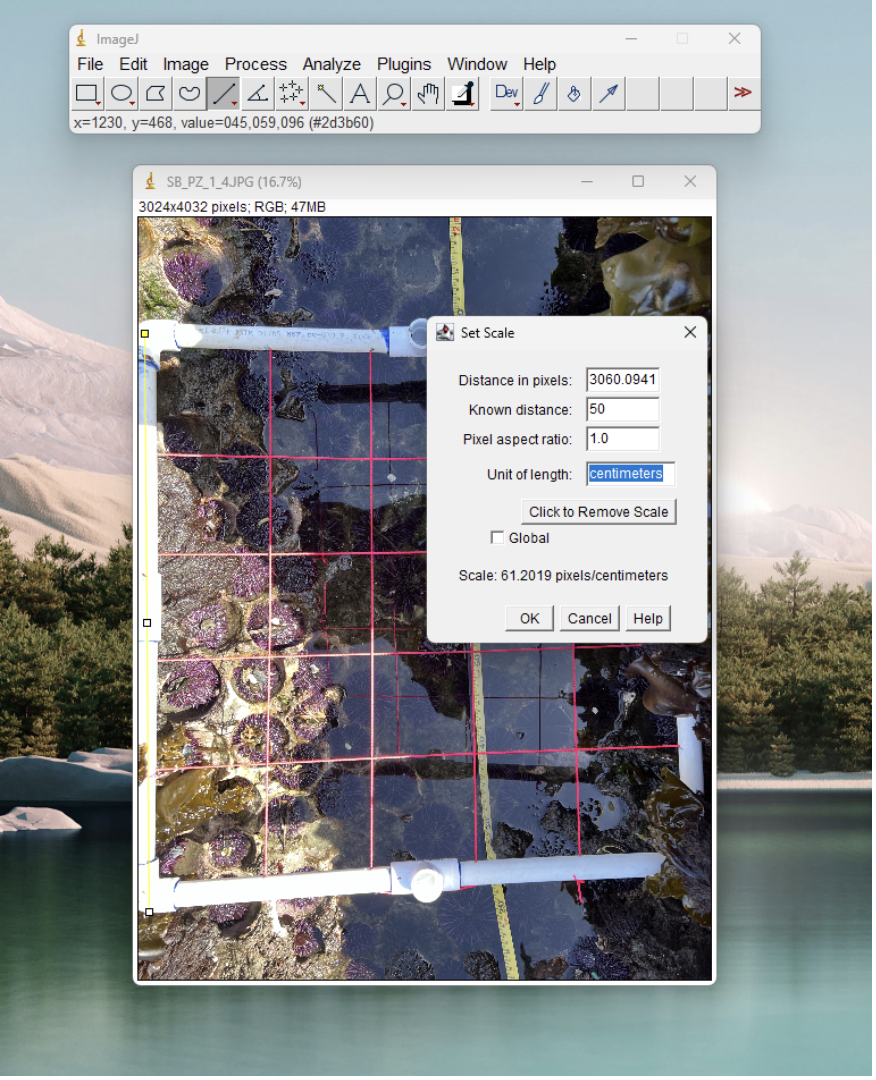
\includegraphics[width=1\linewidth]{figs/SetMeasurement.png}
	\caption{Setting the scale.}
	\label{fig:logo}
\end{figure}


\subsection{Set the measurement to area}

Go to Analyze and Set Measurement. In the Set Measurement window, select Area

\begin{figure}[H]
	\centering
	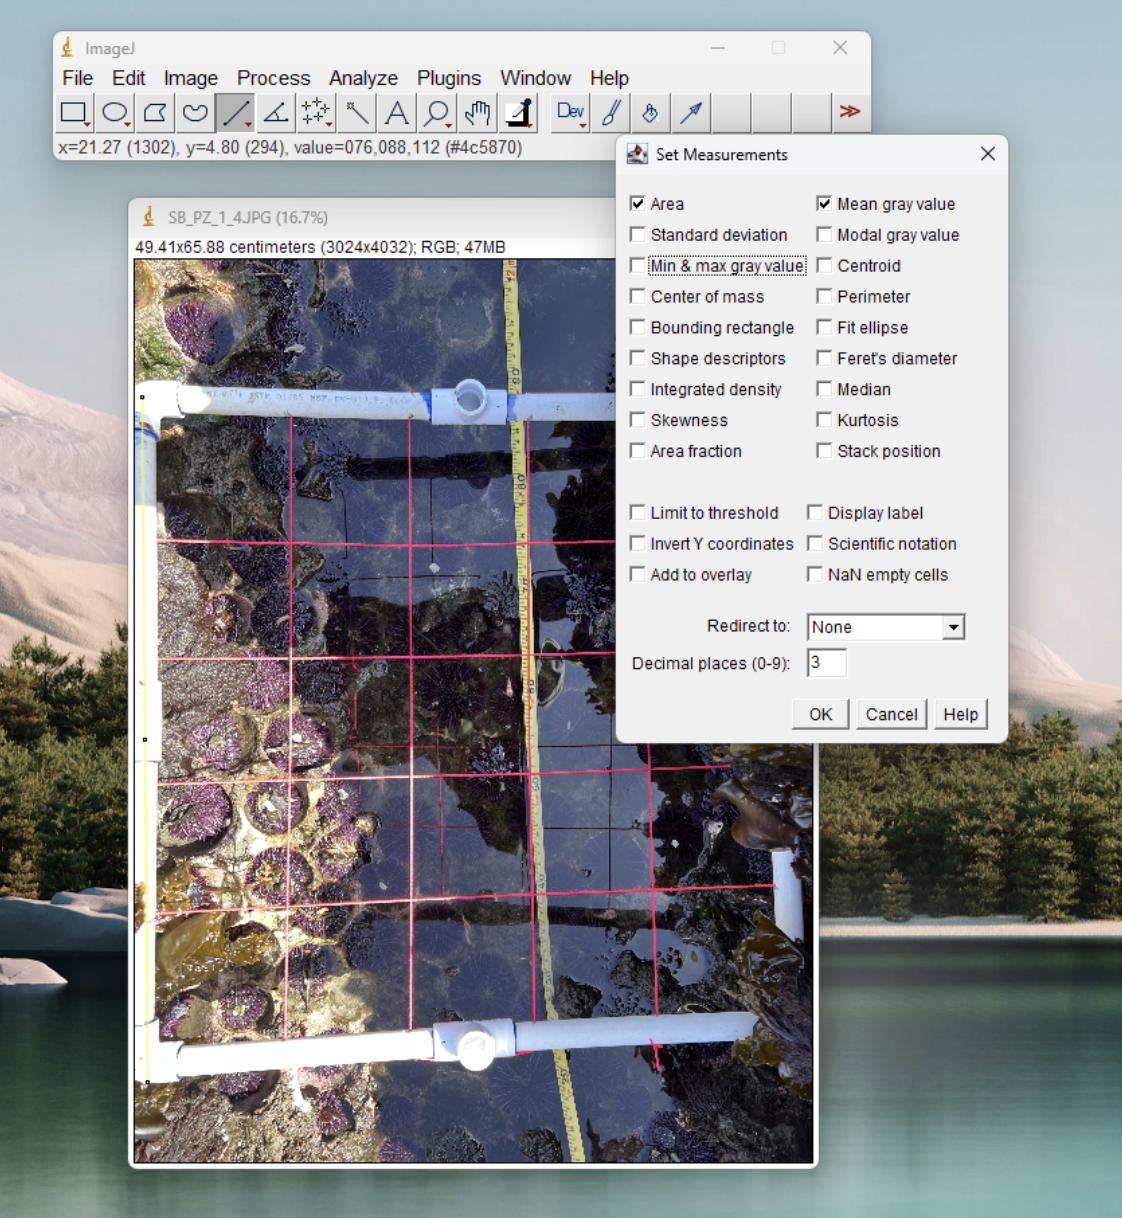
\includegraphics[width=1\linewidth]{figs/SetArea.png}
	\caption{Setting the Area measurements.}
	\label{fig:logo}
\end{figure}


\section{Choosing urchins to measure}

The way you choose which urchins to measure is to pick one relatively in the center of the plot and then one in each of the four corners. This will sort of look like a dice that has been rolled to a 5. If there are urchins only in one region of the plot, then choose urchins closest to each corner and the center. If there are not 5 total urchins, just measure how many are present.  

This way we have some semblance of randomization and we are not biased towards picking the largest urchin.   

\begin{figure}[H]
	\centering
	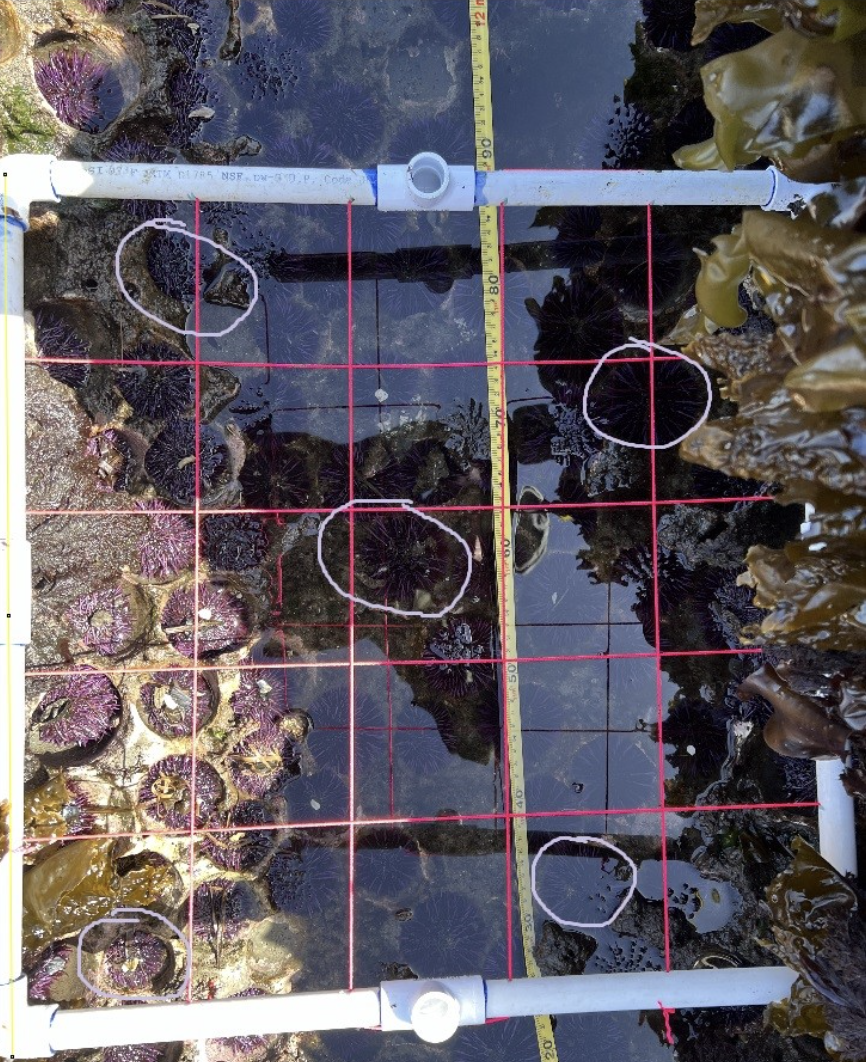
\includegraphics[width=.6\linewidth]{figs/ChoosingUrchins.png}
	\caption{Note here that I selected the urchins I could make our fully. They may not perfectly be in the corner but I wanted to make sure I could reasonably see the urchin.}
	\label{fig:logo}
\end{figure}

\section{Measuring urchins}
\subsection*{Draw a line}

 Draw a line using the line function on the first urchin and then measure the length of the urchin.  
 
\begin{figure}[H]
	\centering
	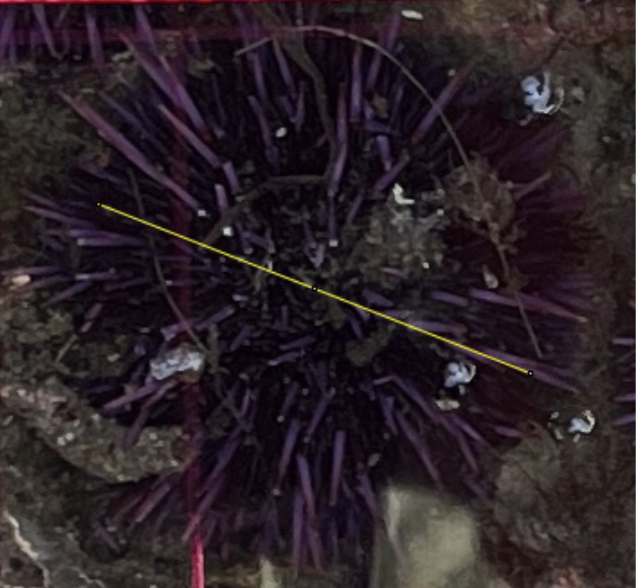
\includegraphics[width=.4\linewidth]{figs/UrchinSize.png}
	\caption{Measure only the test size (not including the spines), or as close as you can get.}
	\label{fig:logo}
\end{figure}

Go to Analyze and Measure. This should open the measurement window and display your length measurement. 

\begin{figure}[H]
	\centering
	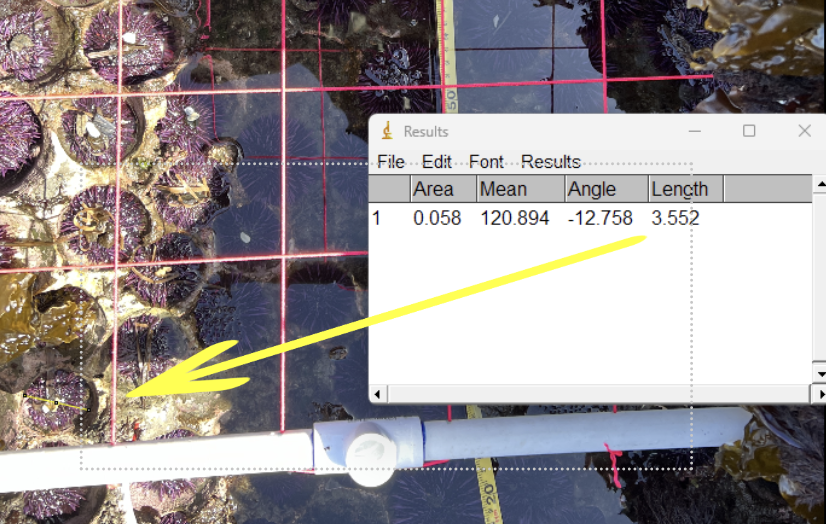
\includegraphics[width=.75\linewidth]{figs/Measure.png}
	\caption{Repeat this for the remaining 4 urchins}
	\label{fig:logo}
\end{figure}

\begin{figure}[H]
	\centering
	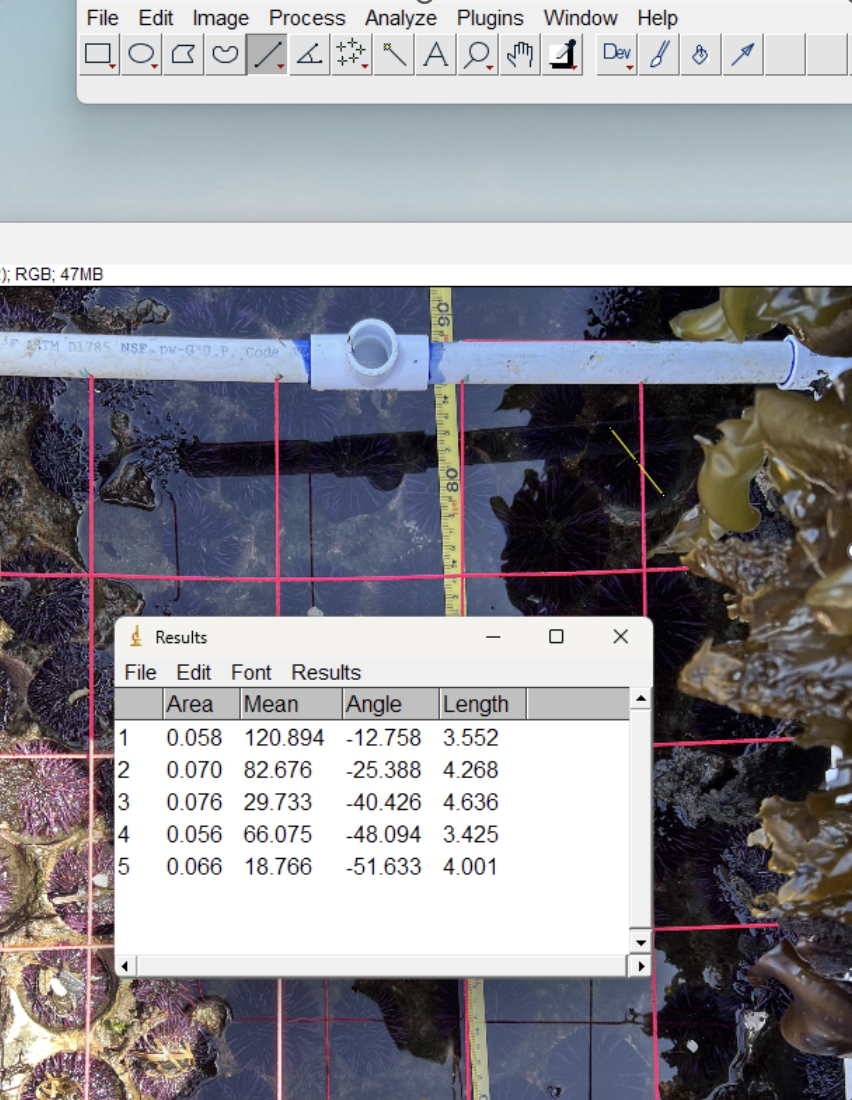
\includegraphics[width=1\linewidth]{figs/AllFive.png}
	\caption{Here are all five measurements from this plot.}
	\label{fig:logo}
\end{figure}

\section{Entering Data}

Input your measurements into the correct lanes in the Excel spreadsheet for each plot. The urchin measurements will have a lavender background.  

You just want to report the length for each urchin.  

Usually, urchins are somewhere between 3 and 10cm in length. If they are crazy big or teensy tinsy- check that your calibration is correct.  

In the example here, the plot was SB PZ14. I have entered it here by rounding to the nearest tenth of a centimeter.  

\begin{figure}[H]
	\centering
	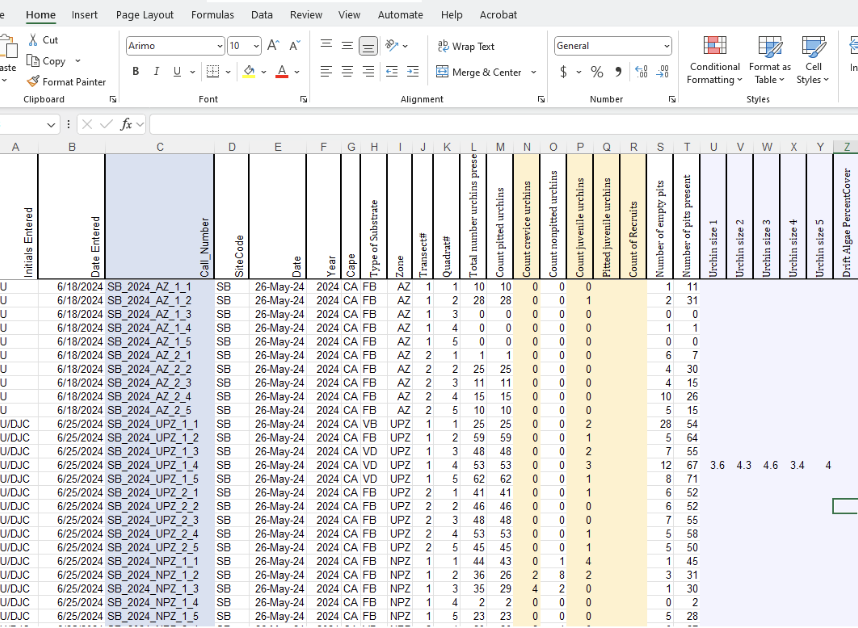
\includegraphics[width=1\linewidth]{figs/IntoExcel.png}
	\caption{}
	\label{fig:logo}
\end{figure}



\end{document}
